We applied the \textit{Cognitive Task Analysis} (CTA) methodology to explore individuals' knowledge and thought processes. Among the various CTA methodologies available, we selected \textit{Goal-Directed Task Analysis} (GDTA), specifically focusing on Situation Awareness (SA) and the goals inherent in SA processes.

GDTA is tailored to identify user goals, the decisions they make, and the critical information needed to achieve these goals. This methodology not only maps out user objectives but also provides insights into their decision-making strategies and information requirements.

By employing GDTA, our aim is to deepen our understanding of how users perceive and interact with information. This understanding informs our design process, ensuring that our solutions align closely with user needs and preferences. Ultimately, this approach enhances the usability and effectiveness of our project outcomes by prioritizing User-Centric design principles.

\section{Initial GDTA Goal Tree}
The initial GDTA Goal Tree, shown in Figure 4.1, identified three Major-Goals. However, after an in-depth review and analysis, we concluded that the Major-Goal 1 \textbf{"Identify prior knowledge in the field of Cybersecurity"} can be integrated into the Major-Goal 2 \textbf{"Define and evaluate the knowledge required for Offensive Cybersecurity by monitoring students' progress"}. This conclusion was drawn from a comprehensive analysis of the sub-goals associated with Major-Goal 1.

Upon examining the sub-goals of Major-Goal 1, it became evident that both the sub-goals and the Major-Goal itself address topics that students need to master throughout their learning journey in cybersecurity. Given that Major-Goal 2 aims to delineate the specific topics and skills students must acquire, we decided to incorporate Major-Goal 1 as a sub-goal within Major-Goal 2. This integration ensures a more cohesive framework for evaluating and defining the necessary knowledge for Offensive Cybersecurity.

Furthermore, the sub-goals of Major-Goal 1 have been reclassified as Level 2 elements, signifying their importance in the comprehension phase of the learning process. 

\begin{figure}[H]
    \centering
    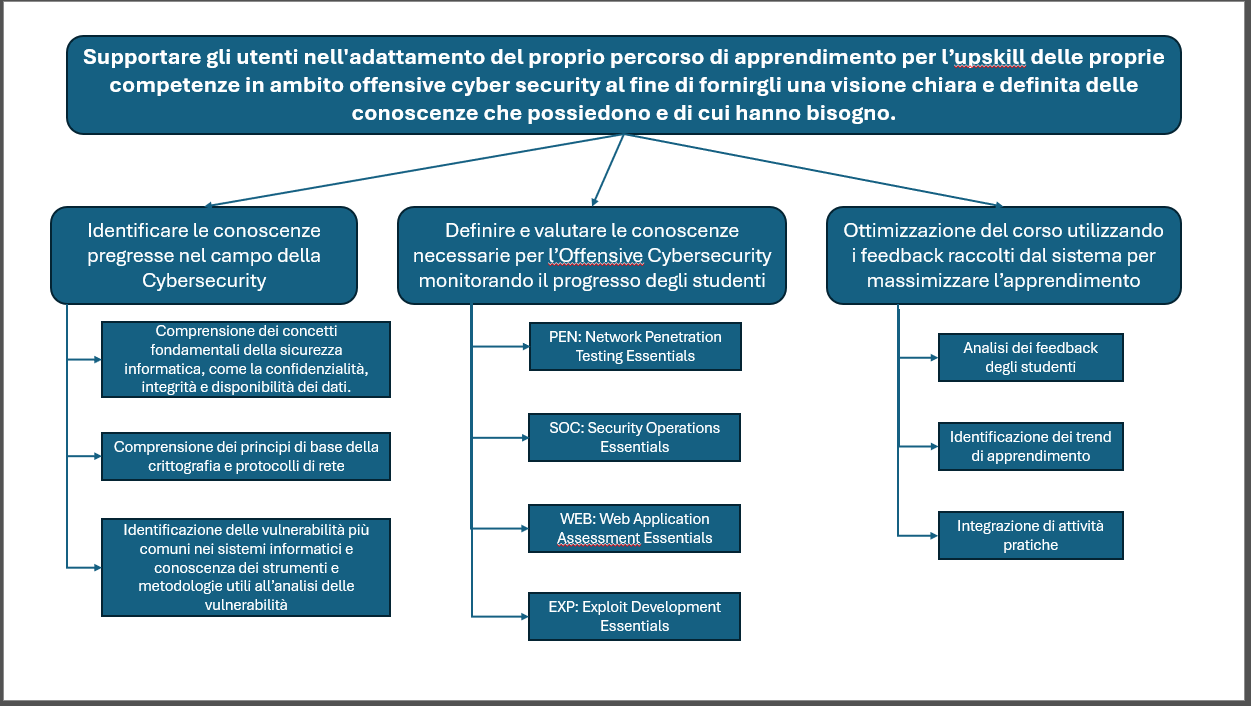
\includegraphics[width=\textwidth]{./assets/GDTA-vecchia.png}
    \caption{Initial GDTA Goal Tree}
    \label{fig:GDTA}
\end{figure}

\newpage
\section{Final GDTA Goal Tree}
In Figure 4.2, we present our Final GDTA Goal Tree, which outlines the primary goals of the system and the sub-goals that contribute to their achievement. In particular, our GDTA Goal Tree supports users in adapting their learning paths to enhance their expertise in Offensive Cybersecurity.
The \textit{Overall Operator Goal} is broken down into two primary \textit{Major-Goals} as shown in the picture below. Each Major-Goal is further divided into \textit{Sub-Goals} that are essential for achieving the Major-Goals. 

\begin{figure}[H]
    \centering
    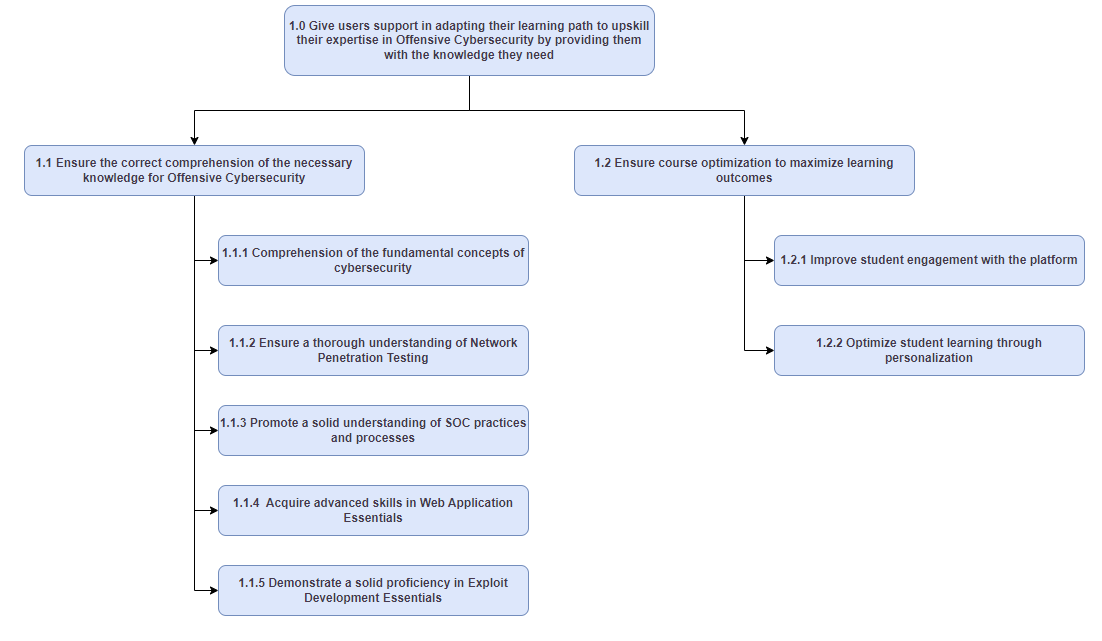
\includegraphics[width=\textwidth]{./assets/GDTA.png}
    \caption{Final GDTA Goal Tree}
    \label{fig:GDTA}
\end{figure}

The following sections will delve into the details of each sub-goal, providing a comprehensive understanding of the cognitive processes involved in achieving these objectives, rather than focusing on the methods or actions needed.
Achieving these goals necessitates more complex cognitive processes than simply searching for a single piece of information.

Subsequently, we defined the \textit{Informational Requirements} for each goal, which are crucial for users to make informed decisions and achieve their objectives. While these requirements might be mistakenly viewed as lower-level goals within the hierarchy, they actually serve as supportive elements that facilitate the achievement of primary goals.

In order to fulfill a goal, a decision must be made based on the available information. We are not interested in trivial yes-or-no questions: instead, we are focusing on decisions that enable the fulfillment of high-level goals. Moreover, these decisions require complex cognitive processes and a deep understanding of the situation.

\newpage
\section{Major-Goal 1.1: Ensure the correct comprehension of the necessary knowledge for Offensive Cybersecurity}
This Major-Goal ensures that users build a solid foundation and understanding of essential cybersecurity concepts and practices. It is divided into five sub-goals.

\subsection{Sub-Goal 1.1.1: Comprehension of the fundamental concepts of cybersecurity }
Users need to grasp the basic principles of cybersecurity, including understanding types of threats, attack vectors, defense mechanisms, and the importance of cybersecurity in protecting information and infrastructure.
The decision associated with subgoal 1.1.1 and its SA requirements are shown in the following figures.
\begin{figure}[H]
    \centering
    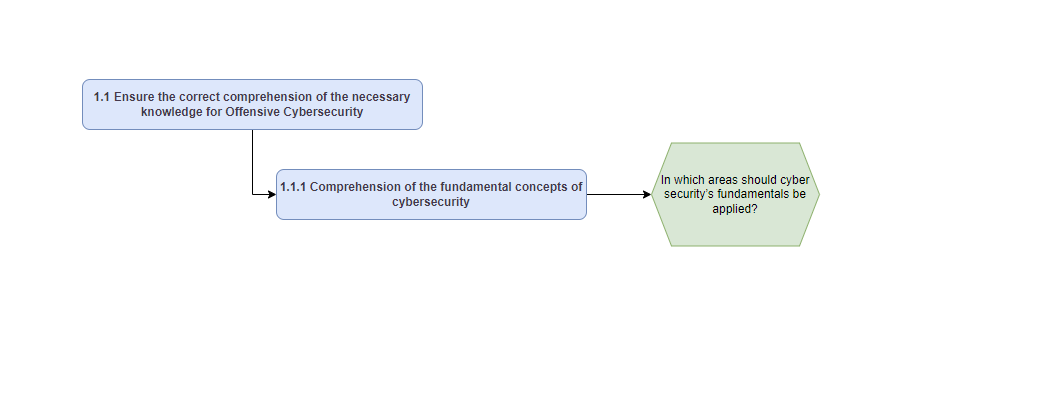
\includegraphics[width=\textwidth]{./assets/subgoal_1.1.1.png}
    \caption{SA Requirements for Sub-Goal 1.1.1}
    \label{fig:subgoal_1.1.1}
\end{figure}

\begin{table}[H]
    \begin{center}
    \begin{tabular}{ | m{5cm} | m{5cm}| m{5cm} | } 
      \hline
      \textbf{Level 1 SA requirements} & \textbf{Level 2 SA requirements}  & \textbf{Level 3 SA requirements}  \\ 
      \hline
      OTP & Confidentiality & Capability to critically evaluate emerging technologies in relation to IT security, current laws and regulations\\ 
      \hline
      SHA256 & Integrity & \\ 
      \hline
      MAC & Confidentiality & \\ 
      \hline
      Digital Signature & Availability  & \\ 
      \hline
      Blockchain & Threat Models  & \\ 
      \hline
      TLS Protocol & Algorithms for Cybersecurity & \\ 
      \hline
    \end{tabular}
    \end{center}
    \caption{SA requirements for subgoal 1.1.1}
    \end{table}
    
\newpage
\subsection{Sub-Goal 1.1.2: Ensure a thorough understanding of Network Penetration Testing}
This involves training users to conduct network penetration tests, which include identifying vulnerabilities within a network, exploiting those vulnerabilities, and providing recommendations to mitigate risks. Users learn about various tools and techniques used in network penetration testing.
The decision associated with subgoal 1.1.2 and its SA requirements are shown in the following figures.
\begin{figure}[H]
    \centering
    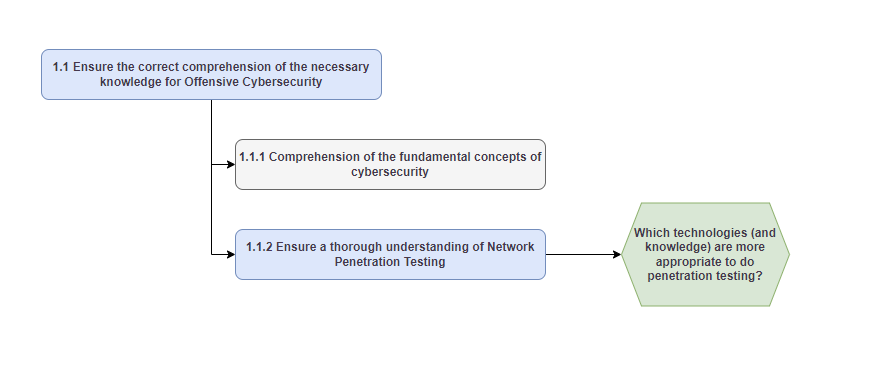
\includegraphics[width=\textwidth]{./assets/subgoal_1.1.2.png}
    \caption{SA Requirements for Sub-Goal 1.1.2}
    \label{fig:subgoal_1.1.2}
\end{figure}

\begin{table}[H]
    \begin{center}
    \begin{tabular}{ | m{5cm} | m{5cm}| m{5cm} | } 
      \hline
      \textbf{Level 1 SA requirements} & \textbf{Level 2 SA requirements}  & \textbf{Level 3 SA requirements}  \\ 
      \hline
      Python operators & Cryptography techniques and hashing & Capability to choose the best penetration testing strategies based on the situation\\ 
      \hline
      Python syntax & Windows networking knowledge & \\ 
      \hline
      Powershell Scripting & Usage of variables & \\ 
      \hline
      Internet Protocol & Loops and functions in Python and Powershell  & \\ 
      \hline
      Domain Name System &  & \\ 
      \hline
    \end{tabular}
    \end{center}
    \caption{SA requirements for subgoal 1.1.2}
    \end{table}
    